
{
    The \textbf{\ac{YOLOv8n}} model\footnote{\ac{YOLOv8n} still does not have a paper for citation. The proper citation before their publication refers to the Ultralytics GitHub page\cite{Jocher_YOLO_by_Ultralytics_2023}.}, with approximately 3.2 million parameters, is a key component of this research. 
    It implements a non-linear mathematical expression without any real meaning but enough complexity to solve \textbf{detection} problems, its true significance emerges after rigorous training. 
    This model is structured around a backbone module, consisting of five levels. 
    Each level becomes progressively smaller in spatial dimensions while incorporating richer features. 
    The output from the last three levels serves as the input for the following pyramidal model.
}

{
    YOLOv8n employs a pyramidal model to process the output from each level effectively. 
    This processing stage leverages contextual information from both lower and higher-level features, enhancing the model's understanding of the input data when locating the detections.
}

{
    Towards the final stage of the model, each level independently generates an output within a detection head. 
    These detections are subject to post-processing techniques, primarily focused on suppressing highly overlapped detection results.
}

%{
%    The various components and their interconnection can be seen on Figure \ref{fig:yolov8_diagram}.
%}

{
    This model was included in this project due to its simplicity for deployment and training through the Ultralytics library\cite{Jocher_YOLO_by_Ultralytics_2023}. 
    The specific rationale behind its selection and its role will be elaborated in the methodology section.
}

%\begin{figure}[!p]
%    \centering
%    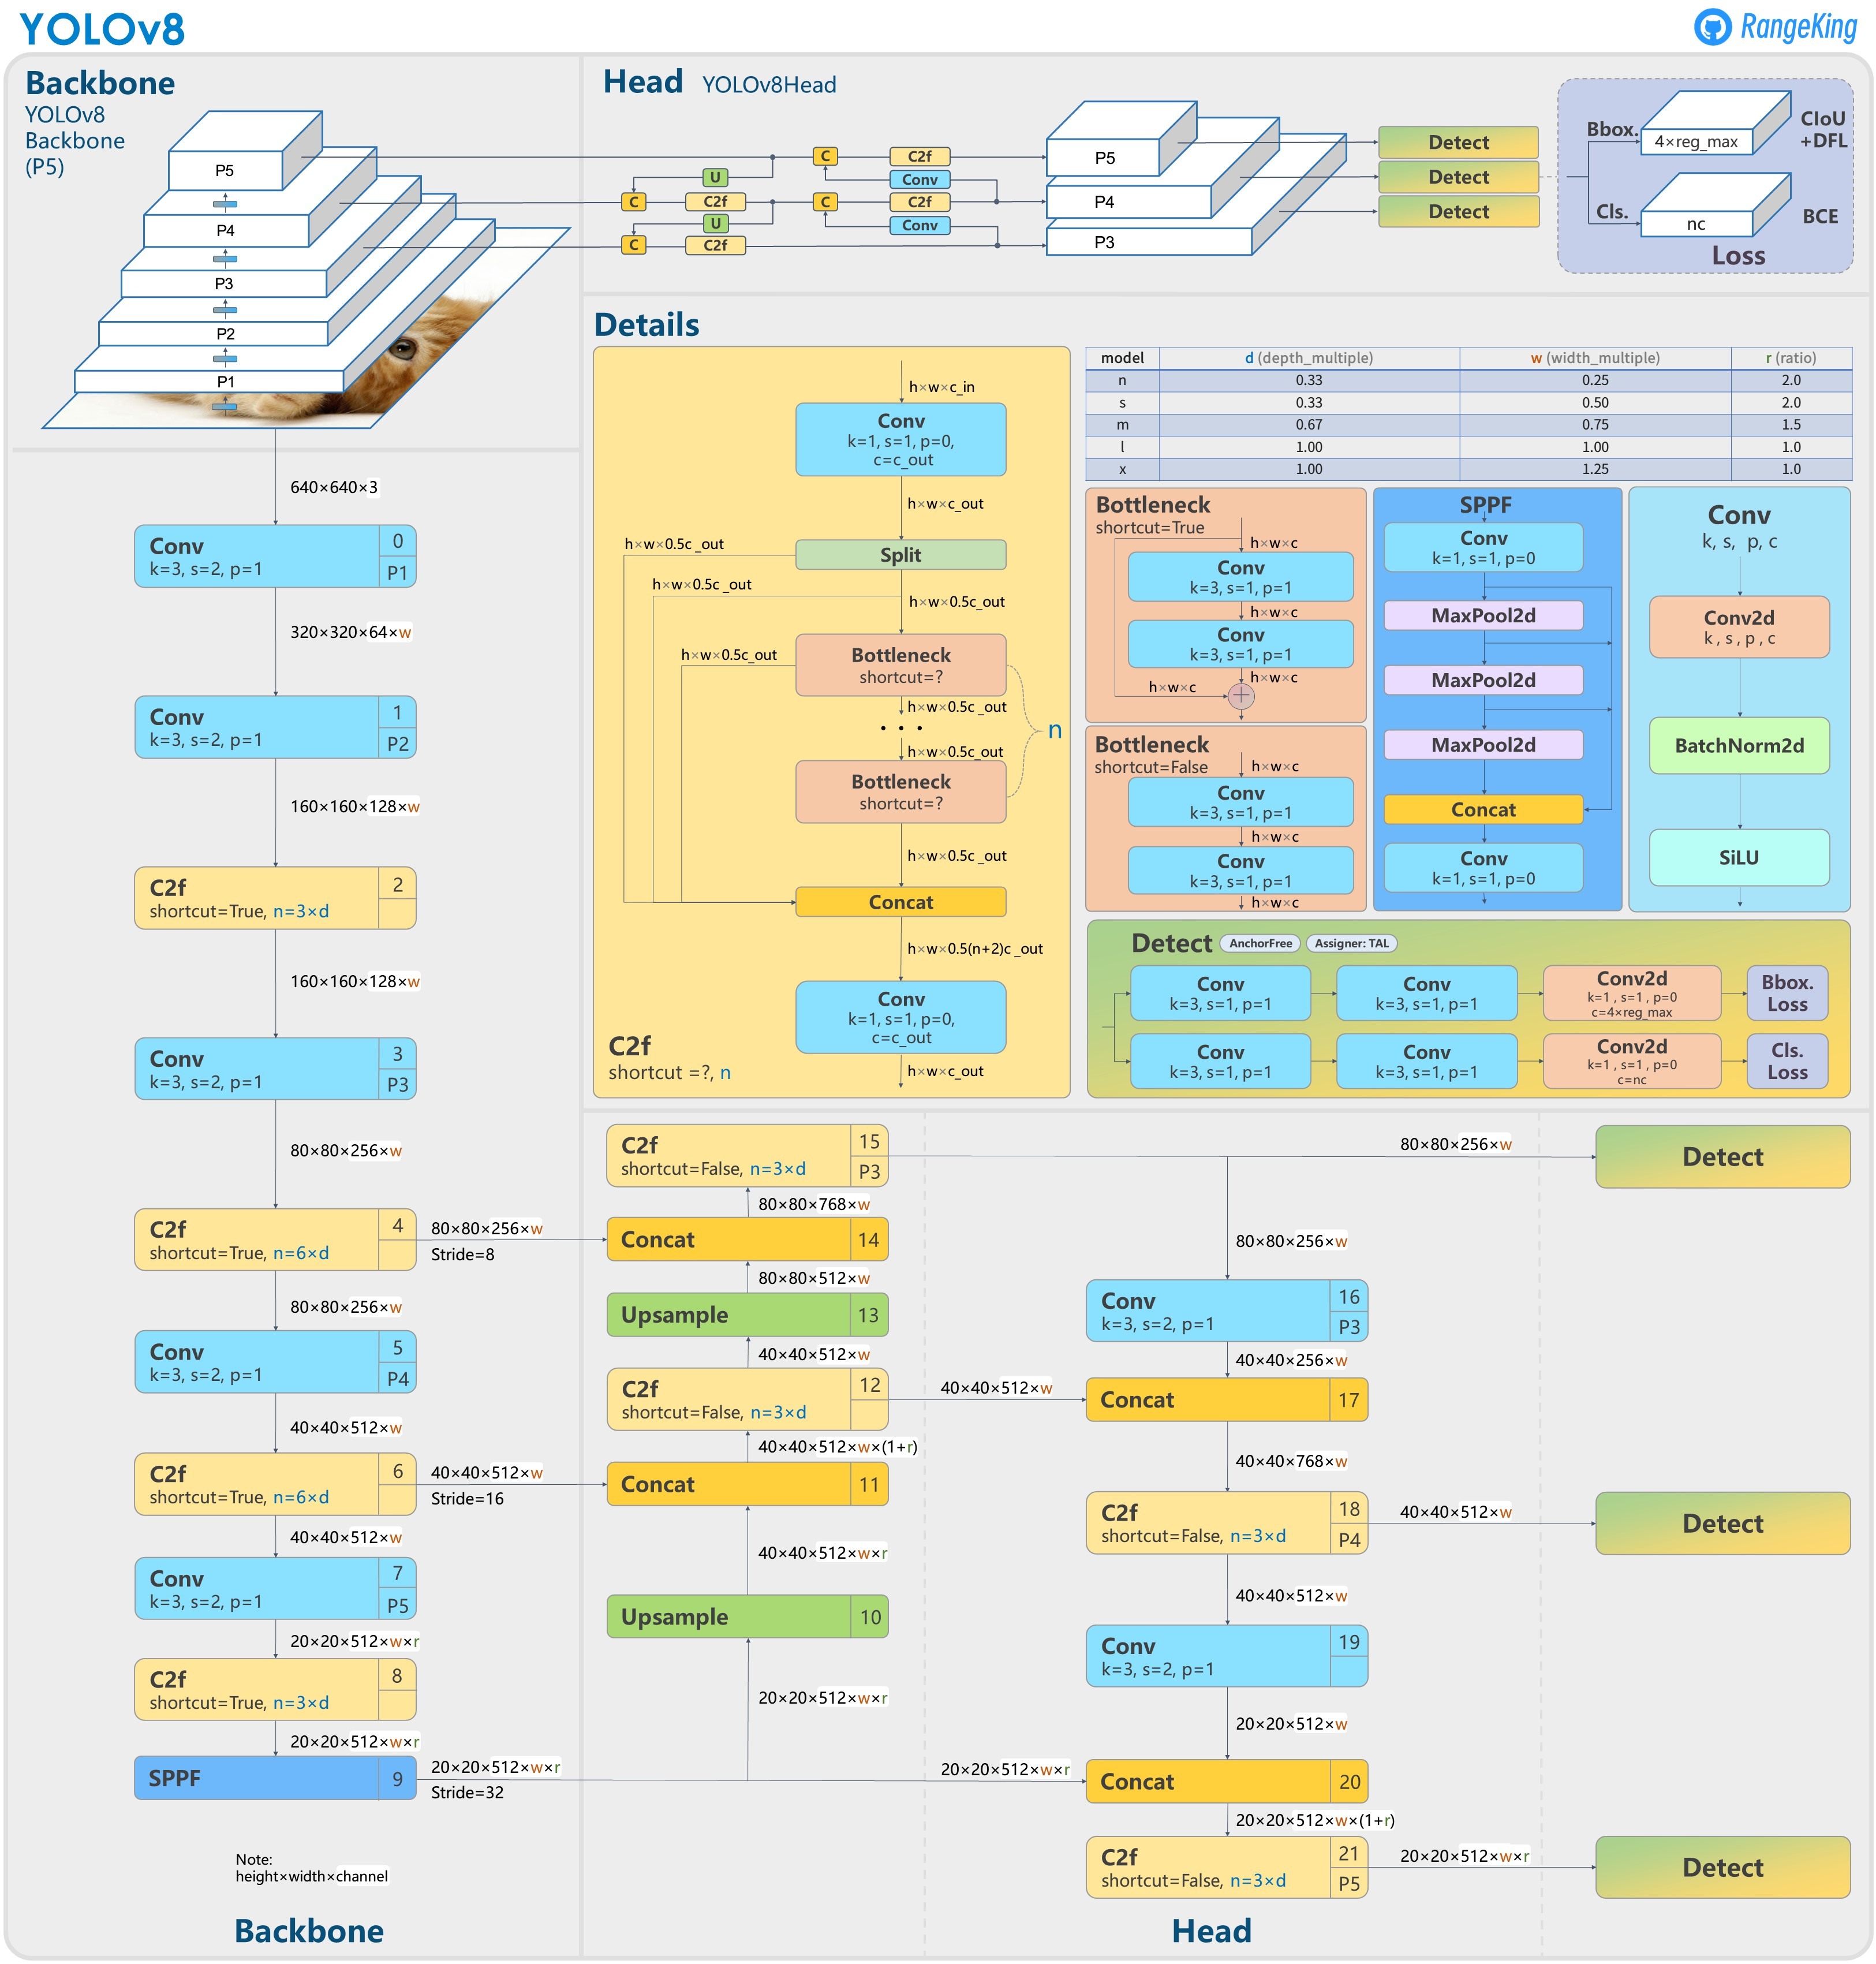
\includegraphics[width=\linewidth]{figures/05_methodology/YOLOv8Diagram.jpg}
%    \caption[YOLOv8 architecture block diagram]{\footnotesize{
%            Block diagram of the \ac{YOLOv8} architecture extracted from an issue on Ultralytics' GitHub from the user RangeKing\cite{YOLOv8_diagram}.
%        }}
%    \label{fig:yolov8_diagram}
%\end{figure}
